\subsection{Progettazione di dettaglio e codifica}
\textit{\textbf{Periodo}: dal 2021-03-08 al 2021-04-09}

L'inizio di questa fase coincide con data della revisione di progettazione e conclude con la scadenza della revisione di qualifica.

\subsubsection{Attività}

\begin{itemize}
\item \textbf{Incremento e verifica documenti}: ;
\item \textbf{Product baseline}: ;
\item \textbf{Allegato tecnico}: ;
\item \textbf{Manuali}: ;
\item \textbf{Consolidamento}: viene realizzata la presentazione da esporre in sede di revisione di qualifica e si approfondiscono aspetti lacunari riguardo il progetto.
\end{itemize}

\subsubsection{Periodi}

\begin{itemize}
\item \textbf{Periodo 1}: \textit{dal 2021-03-8 al 2021-03-11}. \\
Correzione;
\item \textbf{Periodo 2}: \textit{dal 2021-03-11 al 2021-04-02}. \\
Product baseline;
\begin{itemize}
\item \textbf{Incremento 1}: \textit{dal 2021-03-12 al 2021-03-17};
\item \textbf{Incremento 2}: \textit{dal 2021-03-17 al 2021-03-22};
\item \textbf{Incremento 3}: \textit{dal 2021-03-22 al 2021-03-27};
\item \textbf{Incremento 4}: \textit{dal 2021-03-27 al 2021-03-31}.
\end{itemize}
\item \textbf{Periodo 3}: \textit{dal 2021-03-01 al 2021-03-08}. \\
Viene svolta l'attività di consolidamento. Il periodo conclude con la revisione di qualifica;
\end{itemize}

\subsubsection{Diagramma di Gantt}

\begin{figure}[H]
\centering

\centerline{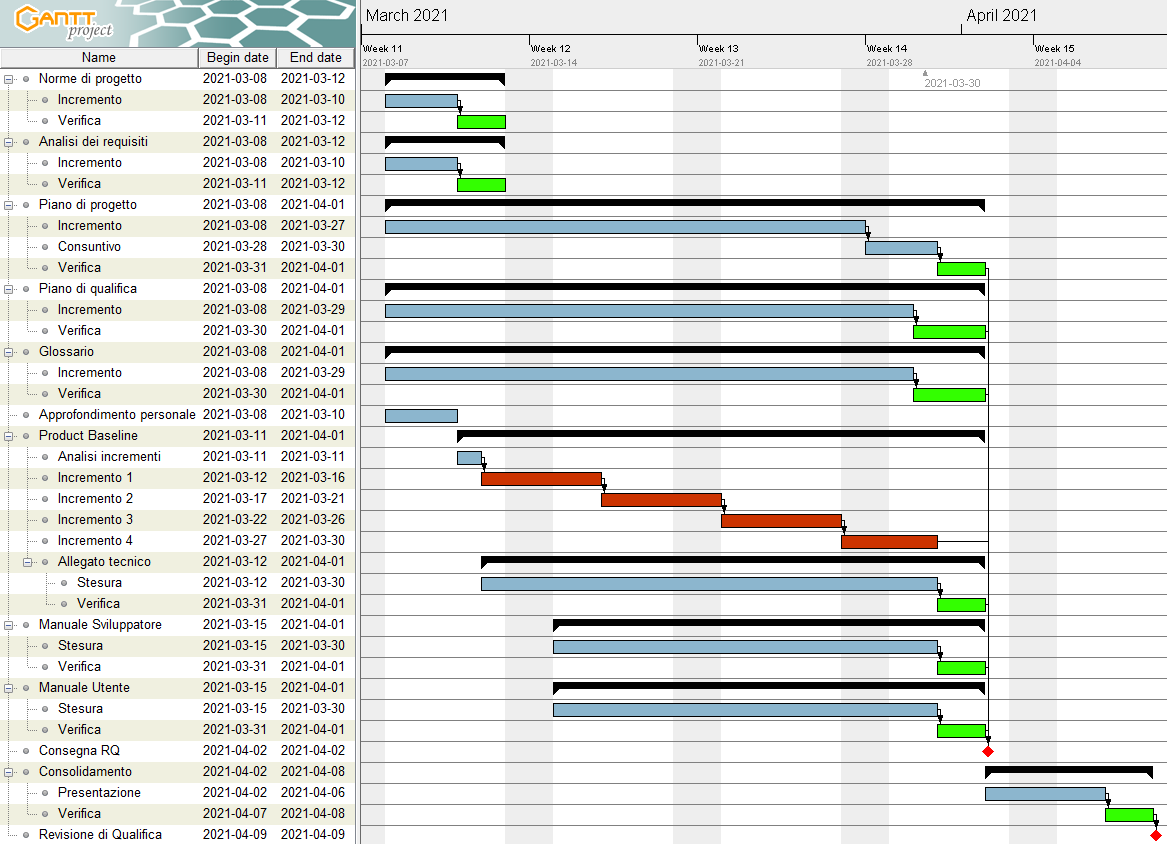
\includegraphics[scale=0.6]{res/Pianificazione/Gantt/codifica}}
\caption{Diagramma di Gantt per il periodo di progettazione di dettaglio e codifica}
\end{figure}

\begin{figure}[H]
\centering

\centerline{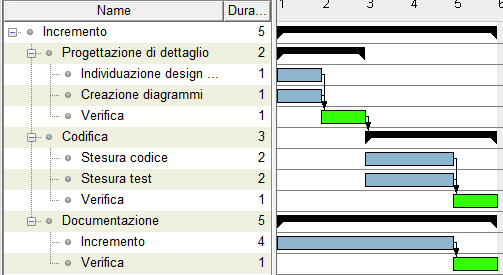
\includegraphics[scale=1]{res/Pianificazione/Gantt/incrementoCodifica}}
\caption{Diagramma di Gantt per i singoli incrementi nel periodo di progettazione di dettaglio e codifica}
\end{figure}
